\RequirePackage{currfile}
\documentclass[12pt]{beamer}
\usepackage[utf8]{inputenc}
\usepackage[spanish]{babel}
\usepackage{standalone}
\usepackage{color}
\usepackage{siunitx}
\usepackage{hyperref}
%\hypersetup{colorlinks,linkcolor=,urlcolor=blue}
%\hypersetup{colorlinks,urlcolor=blue}
\usepackage{xcolor,soul}
\usepackage{etoolbox}
\usepackage{amsmath}
\usepackage{amsthm}
\usepackage{physics}
\usepackage{multicol}
\usepackage{bookmark}
\usepackage{longtable}
\usepackage{listings}
\lstset{
basicstyle=\ttfamily,
columns=fullflexible,
breaklines=true
}
\usepackage{graphicx}
\usepackage{tikz}
\usetikzlibrary{matrix, backgrounds, decorations,shapes, arrows.meta}
\usepackage[autostyle,spanish=mexican]{csquotes}
\usepackage[os=win]{menukeys}
\usepackage{pifont}
\usepackage{pbox}
\usepackage{caption}
\captionsetup{font=scriptsize,labelfont=scriptsize}
\usepackage{dcolumn}
\newcolumntype{L}{D{.}{.}{2,5}}

\definecolor{ao}{rgb}{0.0, 0.5, 0.0}
\definecolor{bisque}{rgb}{1.0, 0.89, 0.77}
\definecolor{amber}{rgb}{1.0, 0.75, 0.0}
\definecolor{armygreen}{rgb}{0.29, 0.33, 0.13}
\definecolor{alizarin}{rgb}{0.82, 0.1, 0.26}
\definecolor{cadetblue}{rgb}{0.37, 0.62, 0.63}
\definecolor{deepblue}{rgb}{0,0,0.5}
\definecolor{brown}{rgb}{0.59, 0.29, 0.0}
\definecolor{OliveGreen}{rgb}{0,0.25,0}

\definecolor{Code}{rgb}{0,0,0}
\definecolor{Keywords}{rgb}{255,0,0}
\definecolor{Strings}{rgb}{255,0,255}
\definecolor{Comments}{rgb}{0,0,255}
\definecolor{Numbers}{rgb}{255,128,0}


\newcommand*{\TitleParbox}[1]{\parbox[c]{1.75cm}{\raggedright #1}}%

%\usepackage[sfdefault]{roboto}  %% Option 'sfdefault' only if the base font of the document is to be sans serif

\renewcommand{\arraystretch}{1.5}
\renewcommand{\rmdefault}{cmr}% cmr = Computer Modern Roman
\usefonttheme[onlymath]{serif}

\newcommand{\python}{\texttt{python}}
\newcommand{\textoazul}[1]{\textcolor{blue}{#1}}
\newcommand{\azulfuerte}[1]{\textcolor{blue}{\textbf{#1}}}
\newcommand{\funcionazul}[1]{\textcolor{blue}{\textbf{\texttt{#1}}}}

\newcounter{saveenumi}
\newcommand{\seti}{\setcounter{saveenumi}{\value{enumi}}}
\newcommand{\conti}{\setcounter{enumi}{\value{saveenumi}}}

\linespread{1.5}
\beamertemplatenavigationsymbolsempty
\usefonttheme{professionalfonts}
%\usefonttheme{serif}
\DeclareGraphicsExtensions{.pdf,.png,.jpg}
\renewcommand {\arraystretch}{1.25}
\mode<presentation>
{
  \usetheme{Warsaw}
  \setbeamertemplate{headline}{}
  %\useoutertheme{infolines}
  \useoutertheme{default}
  \setbeamercovered{invisible}
  % or whatever (possibly just delete it)
  \setbeamertemplate{section in toc}[sections numbered]
  \setbeamertemplate{subsection in toc}[subsections numbered]
  \setbeamertemplate{subsection in toc}{\leavevmode\leftskip=3.2em\rlap{\hskip-2em\inserttocsectionnumber.\inserttocsubsectionnumber}\inserttocsubsection\par}
  \setbeamercolor{section in toc}{fg=blue}
  \setbeamercolor{subsection in toc}{fg=blue}
  \setbeamercolor{frametitle}{fg=yellow}

  \setbeamertemplate{footline} 
{
  \leavevmode%
  \hbox{%
  \begin{beamercolorbox}[wd=.333333\paperwidth,ht=2.25ex,dp=1ex,center]{author in head/foot}%
    \usebeamerfont{author in head/foot}\insertsection
  \end{beamercolorbox}%
  \begin{beamercolorbox}[wd=.333333\paperwidth,ht=2.25ex,dp=1ex,center]{title in head/foot}%
    \usebeamerfont{title in head/foot}\textcolor{yellow}{\insertsubsection}
  \end{beamercolorbox}%
  \begin{beamercolorbox}[wd=.333333\paperwidth,ht=2.25ex,dp=1ex,right]{date in head/foot}%
    \usebeamerfont{date in head/foot}\insertshortdate{}\hspace*{2em}
    \insertframenumber{} / \inserttotalframenumber\hspace*{2ex} 
  \end{beamercolorbox}}%
  \vskip0pt%
}
}
\makeatother

\makeatletter
\patchcmd{\beamer@sectionintoc}
  {\vfill}
  {\vskip\itemsep}
  {}
  {}
\makeatother

% \makeatletter
% \patchcmd{\hyper@link@}
%   {{\Hy@tempb}{#4}}
%   {{\Hy@tempb}{\ul{#4}}}
%   {}{}
% \makeatother

\DeclareCaptionFont{white}{\color{white}}
\DeclareCaptionFormat{listing}{\colorbox{gray}{\parbox{0.99\textwidth}{#1#2#3}}}
\captionsetup[lstlisting]{format=listing,labelfont=white,textfont=white}
\renewcommand{\lstlistingname}{Código}

\lstdefinestyle{codigopython}{%
  language=Python,                % choose the language of the code
  %basicstyle=\footnotesize\small,       % the size of the fonts that are used for the code
  numbers=left,                   % where to put the line-numbers
  numberstyle=\scriptsize,      % the size of the fonts that are used for the line-numbers
  stepnumber=1,                   % the step between two line-numbers. If it is 1 each line will be numbered
  numbersep=5pt,                  % how far the line-numbers are from the code
  backgroundcolor=\color{white},  % choose the background color. You must add \usepackage{color}
  showspaces=false,               % show spaces adding particular underscores
  showstringspaces=false,         % underline spaces within strings
  showtabs=false,                 % show tabs within strings adding particular underscores
  frame=single,   		% adds a frame around the code
  tabsize=2,  		% sets default tabsize to 2 spaces
  captionpos=t,   		% sets the caption-position to bottom
  breaklines=true,    	% sets automatic line breaking
  breakatwhitespace=false,    % sets if automatic breaks should only happen at whitespace
  escapeinside={\#},  % if you want to add a comment within your code
  stringstyle =\color{OliveGreen},
  texcl = true,
  %otherkeywords={{as}},             % Add keywords here
  keywordstyle = \color{blue},
  commentstyle = \color{black},
  identifierstyle = \color{black},
  % literate=%
  %         {á}{{\'a}}1
  %         {é}{{\'e}}1
  %         {í}{{\'i}}1
  %         {ó}{{\'o}}1
  %         {ú}{{\'u}}1
  %
  %keywordstyle=\ttb\color{deepblue}
  %fancyvrb = true,
literate={0}{{\textcolor{red}{0}}}{1}%
            {1}{{\textcolor{red}{1}}}{1}%
            {2}{{\textcolor{red}{2}}}{1}%
            {3}{{\textcolor{red}{3}}}{1}%
            {4}{{\textcolor{red}{4}}}{1}%
            {5}{{\textcolor{red}{5}}}{1}%
            {6}{{\textcolor{red}{6}}}{1}%
            {7}{{\textcolor{red}{7}}}{1}%
            {8}{{\textcolor{red}{8}}}{1}%
            {9}{{\textcolor{red}{9}}}{1}%
            {.0}{{\textcolor{red}{.0}}}{2}% Following is to ensure that only periods
            {.1}{{\textcolor{red}{.1}}}{2}% followed by a digit are changed.
            {.2}{{\textcolor{red}{.2}}}{2}%
            {.3}{{\textcolor{red}{.3}}}{2}%
            {.4}{{\textcolor{red}{.4}}}{2}%
            {.5}{{\textcolor{red}{.5}}}{2}%
            {.6}{{\textcolor{red}{.6}}}{2}%
            {.7}{{\textcolor{red}{.7}}}{2}%
            {.8}{{\textcolor{red}{.8}}}{2}%
            {.9}{{\textcolor{red}{.9}}}{2}%
            {\ }{{ }}{1}% handle the space
        ,%
        %mathescape=true
        %escapeinside={*@}
        escapeinside={A_}{_B}
}


%%\RequirePackage[l2tabu, orthodox]{nag}
\RequirePackage{currfile}
\documentclass[12pt]{beamer}
\graphicspath{{Imagenes/}{../Imagenes/}}
\usepackage[utf8]{inputenc}
\usepackage[spanish]{babel}
\usepackage{standalone}
\usepackage{color}
\usepackage[binary-units=true]{siunitx}
\usepackage{hyperref}
\hypersetup{
  colorlinks=true,
  linkcolor=blue,          % color of internal links (change box color with linkbordercolor)
  citecolor=green,        % color of links to bibliography
  filecolor=magenta,      % color of file links
  urlcolor=cyan,           % color of external links
  linkbordercolor={0 0 1}
}
\usepackage{xcolor, soul}
\usepackage{etoolbox}
\usepackage{amsmath}
\usepackage{amsthm}
\usepackage{physics}
\usepackage{multicol}
\usepackage{graphicx}
\usepackage{bookmark}
\usepackage{longtable}
\usepackage{graphicx}
\usepackage{tikz}
\usepackage[siunitx, RPvoltages]{circuitikz}
\usetikzlibrary{mindmap}
\usetikzlibrary{arrows, patterns, shapes, decorations.markings, decorations.pathmorphing}
\usetikzlibrary{matrix,positioning}
\tikzstyle{every picture}+=[remember picture,baseline]
\usepackage[autostyle,spanish=mexican]{csquotes}
\usepackage{pifont}
\usepackage[font=footnotesize,textfont=it]{caption}
\usepackage{tabulary}
\usepackage{booktabs}
\usepackage[outdir=./]{epstopdf}
%\usepackage{epstopdf}
\usepackage{media9}
\usepackage{multimedia}
\usepackage{bigints}
%\usepackage{enumitem}
\usepackage[os=win]{menukeys}
\usepackage{pifont}
\usepackage{pbox}
\usepackage{alltt}
\usepackage{verbatim}
\usepackage{colortbl}
\usepackage{tcolorbox}
\usepackage{fancyvrb}
\usepackage[sfdefault]{roboto}  %% Option 'sfdefault' only if the base font of the document is to be sans serif
%\usepackage[T1]{fontenc}
\setcounter{secnumdepth}{3}
\setcounter{tocdepth}{3}
\DeclareGraphicsExtensions{.pdf,.png,.jpg}
\renewcommand {\arraystretch}{1.5}
\definecolor{ao}{rgb}{0.0, 0.5, 0.0}
\definecolor{aquamarine}{rgb}{0.5, 1.0, 0.83}
\definecolor{kellygreen}{rgb}{0.3, 0.73, 0.09}
\definecolor{bisque}{rgb}{1.0, 0.89, 0.77}
\definecolor{amber}{rgb}{1.0, 0.75, 0.0}
\definecolor{armygreen}{rgb}{0.29, 0.33, 0.13}
\definecolor{alizarin}{rgb}{0.82, 0.1, 0.26}
\definecolor{cadetblue}{rgb}{0.37, 0.62, 0.63}
\newcommand*{\TitleParbox}[1]{\parbox[c]{6cm}{\raggedright #1}}%
\newcommand{\python}{\texttt{python}}
\newcommand{\textoazul}[1]{\textcolor{blue}{#1}}
\newcommand{\azulfuerte}[1]{\textcolor{blue}{\textbf{#1}}}
\newcommand{\funcionazul}[1]{\textcolor{blue}{\textbf{\texttt{#1}}}}
%\normalfont
\usepackage{ccfonts}% http://ctan.org/pkg/{ccfonts}
\usepackage[T1]{fontenc}% http://ctan.or/pkg/fontenc
\renewcommand{\rmdefault}{cmr}% cmr = Computer Modern Roman
\usefonttheme[onlymath]{serif}
\linespread{1.3}
\newcounter{saveenumi}
\newcommand{\seti}{\setcounter{saveenumi}{\value{enumi}}}
\newcommand{\conti}{\setcounter{enumi}{\value{saveenumi}}}
\newcommand{\tikzmark}[1]{\tikz[remember picture] \node[coordinate] (#1) {#1};}

\usepackage{scalerel}[2016-12-29]
\def\stretchint#1{\vcenter{\hbox{\stretchto[440]{\displaystyle\int}{#1}}}}
\def\scaleint#1{\vcenter{\hbox{\scaleto[3ex]{\displaystyle\int}{#1}}}}
\def\bs{\mkern-12mu}

\newtheorem{teo}{}[section]
\usepackage{blkarray}

%reduce el tamaño de letra de la etiqueta equations
\makeatletter
\def\maketag@@@#1{\hbox{\m@th\normalfont\small#1}}
\makeatother

%se usa para la x en itemize
\newcommand{\xmark}{\text{\ding{55}}}

%\AtBeginDocument{\setlength{\tymin}{1em}}


\definecolor{myblue}{rgb}{.8, .8, 1}

\usepackage{empheq}

\newlength\mytemplen
\newsavebox\mytempbox

\makeatletter
\newcommand\mybluebox{%
    \@ifnextchar[%]
       {\@mybluebox}%
       {\@mybluebox[0pt]}}

\def\@mybluebox[#1]{%
    \@ifnextchar[%]
       {\@@mybluebox[#1]}%
       {\@@mybluebox[#1][0pt]}}

\def\@@mybluebox[#1][#2]#3{
    \sbox\mytempbox{#3}%
    \mytemplen\ht\mytempbox
    \advance\mytemplen #1\relax
    \ht\mytempbox\mytemplen
    \mytemplen\dp\mytempbox
    \advance\mytemplen #2\relax
    \dp\mytempbox\mytemplen
    \colorbox{myblue}{\hspace{1em}\usebox{\mytempbox}\hspace{1em}}}

\makeatother



%\usetheme{CambridgeUS}
%%Se usa la plantilla Warsaw modificada con spruce
\mode<presentation>
{
  \usetheme{Berlin}
  \setbeamertemplate{headline}{}
  \useoutertheme{default}
  \usecolortheme{beaver}
  \setbeamercovered{invisible}
}
%\AtBeginSection[]
%{
%\begin{frame}<beamer>{Contenido}
%\normalfont\mdseries
%\tableofcontents[currentsection]
%\end{frame}
%}

\setbeamertemplate{section in toc}[sections numbered]
\setbeamertemplate{subsection in toc}[subsections numbered]
\setbeamertemplate{subsection in toc}{\leavevmode\leftskip=3.2em\rlap{\hskip-2em\inserttocsectionnumber.\inserttocsubsectionnumber}\inserttocsubsection\par}
\setbeamercolor{section in toc}{fg=blue}
\setbeamercolor{subsection in toc}{fg=blue}
\setbeamertemplate{navigation symbols}{}
\setbeamercolor{frametitle}{fg=amber,bg=armygreen}
%\setbeamercolor{frametitle}{fg=blue,bg=ao!90!white}
\setbeamercolor{section in head/foot}{bg=gray!30,fg=red}
%\setbeamercolor{section in head}{bg=green,fg=red}
\setbeamercolor{subsection in head/foot}{bg=gray!30,fg=black}
\setbeamercolor{author in head/foot}{bg=gray!30}
\setbeamercolor{date in head/foot}{fg=blue}

%\mode<presentation>
%{
%  \usetheme{Warsaw}
%  \setbeamertemplate{headline}{}
%  %\useoutertheme{infolines}
%  \useoutertheme{default}
%  \setbeamercovered{invisible}
%  % or whatever (possibly just delete it)
%}

%\usepackage[backend=biber]{biblatex}
%\bibliography{LibrosFC.bib}
%\usepackage{courier}
\usepackage{listingsutf8}
\usepackage{listings}
\usepackage{xcolor}
\usepackage{textcomp}
\usepackage{color}
\definecolor{deepblue}{rgb}{0,0,0.5}
\definecolor{brown}{rgb}{0.59, 0.29, 0.0}
\definecolor{OliveGreen}{rgb}{0,0.25,0}
% \usepackage{minted}

\DeclareCaptionFont{white}{\color{white}}
\DeclareCaptionFormat{listing}{\colorbox{gray}{\parbox{0.98\textwidth}{#1#2#3}}}
\captionsetup[lstlisting]{format=listing,labelfont=white,textfont=white}
\renewcommand{\lstlistingname}{Código}


\definecolor{Code}{rgb}{0,0,0}
\definecolor{Keywords}{rgb}{255,0,0}
\definecolor{Strings}{rgb}{255,0,255}
\definecolor{Comments}{rgb}{0,0,255}
\definecolor{Numbers}{rgb}{255,128,0}

\makeatletter

\newif\iffirstchar\firstchartrue
\newif\ifstartedbyadigit
\newif\ifprecededbyequalsign

\newcommand\processletter
{%
  \ifnum\lst@mode=\lst@Pmode%
    \iffirstchar%
        \global\startedbyadigitfalse%
      \fi
      \global\firstcharfalse%
    \fi
}

\newcommand\processdigit
{%
  \ifnum\lst@mode=\lst@Pmode%
      \iffirstchar%
        \global\startedbyadigittrue%
      \fi
      \global\firstcharfalse%
  \fi
}

\lst@AddToHook{OutputOther}%
{%
  \lst@IfLastOtherOneOf{=}
    {\global\precededbyequalsigntrue}
    {}%
}

\lst@AddToHook{Output}%
{%
  \ifprecededbyequalsign%
      \ifstartedbyadigit%
        \def\lst@thestyle{\color{orange}}%
      \fi
    \fi
  \global\firstchartrue%
  \global\startedbyadigitfalse%
  \global\precededbyequalsignfalse%
}

\lstset{ 
language=Python,                % choose the language of the code
basicstyle=\footnotesize\ttfamily,       % the size of the fonts that are used for the code
numbers=left,                   % where to put the line-numbers
numberstyle=\scriptsize,      % the size of the fonts that are used for the line-numbers
stepnumber=1,                   % the step between two line-numbers. If it is 1 each line will be numbered
numbersep=5pt,                  % how far the line-numbers are from the code
backgroundcolor=\color{white},  % choose the background color. You must add \usepackage{color}
showspaces=false,               % show spaces adding particular underscores
showstringspaces=false,         % underline spaces within strings
showtabs=false,                 % show tabs within strings adding particular underscores
frame=single,   		% adds a frame around the code
tabsize=2,  		% sets default tabsize to 2 spaces
captionpos=t,   		% sets the caption-position to bottom
breaklines=true,    	% sets automatic line breaking
breakatwhitespace=false,    % sets if automatic breaks should only happen at whitespace
escapeinside={\#},  % if you want to add a comment within your code
stringstyle =\color{OliveGreen},
%otherkeywords={{as}},             % Add keywords here
keywordstyle = \color{blue},
commentstyle = \color{black},
identifierstyle = \color{black},
literate=%
         {á}{{\'a}}1
         {é}{{\'e}}1
         {í}{{\'i}}1
         {ó}{{\'o}}1
         {ú}{{\'u}}1
%
%keywordstyle=\ttb\color{deepblue}
%fancyvrb = true,
}

\lstdefinestyle{FormattedNumber}{%
    literate={0}{{\textcolor{red}{0}}}{1}%
             {1}{{\textcolor{red}{1}}}{1}%
             {2}{{\textcolor{red}{2}}}{1}%
             {3}{{\textcolor{red}{3}}}{1}%
             {4}{{\textcolor{red}{4}}}{1}%
             {5}{{\textcolor{red}{5}}}{1}%
             {6}{{\textcolor{red}{6}}}{1}%
             {7}{{\textcolor{red}{7}}}{1}%
             {8}{{\textcolor{red}{8}}}{1}%
             {9}{{\textcolor{red}{9}}}{1}%
             {.0}{{\textcolor{red}{.0}}}{2}% Following is to ensure that only periods
             {.1}{{\textcolor{red}{.1}}}{2}% followed by a digit are changed.
             {.2}{{\textcolor{red}{.2}}}{2}%
             {.3}{{\textcolor{red}{.3}}}{2}%
             {.4}{{\textcolor{red}{.4}}}{2}%
             {.5}{{\textcolor{red}{.5}}}{2}%
             {.6}{{\textcolor{red}{.6}}}{2}%
             {.7}{{\textcolor{red}{.7}}}{2}%
             {.8}{{\textcolor{red}{.8}}}{2}%
             {.9}{{\textcolor{red}{.9}}}{2}%
             {\ }{{ }}{1}% handle the space
         ,%
          %mathescape=true
          escapeinside={__}
          }



%\setbeamercolor{section in foot}{fg=white, bg=BlueViolet}
\makeatletter
\setbeamertemplate{footline}
{
  \leavevmode%
  \hbox{%
  \begin{beamercolorbox}[wd=.333333\paperwidth,ht=2.25ex,dp=1ex,center]{author in head/foot}%
    \usebeamerfont{section in /foot} {\insertsection}
  \end{beamercolorbox}%
  \begin{beamercolorbox}[wd=.333333\paperwidth,ht=2.25ex,dp=1ex,center]{title in head/foot}%
    \usebeamerfont{section in head/foot} {\insertsubsection}
  \end{beamercolorbox}%
  \begin{beamercolorbox}[wd=.333333\paperwidth,ht=2.25ex,dp=1ex,right]{date in head/foot}%
    \usebeamerfont{date in head/foot}\insertshortdate{}\hspace*{2em}
    \insertframenumber{} / \inserttotalframenumber\hspace*{2ex} 
  \end{beamercolorbox}}%
  \vskip0pt%
}
\makeatother

\title{Tema 0 - Introducción a \python}
%\subtitle{Semestre 2018-2}
\author[]{M. en C. Gustavo Contreras Mayén \\ M. en C. Abraham Lima Buendía}
\institute{Facultad de Ciencias - UNAM}
\titlegraphic{
\includegraphics[width=2cm]{escudo-facultad-ciencias}\hspace*{4.75cm}~%
   
\includegraphics[width=2cm]{escudo-unam}
}
\date{\today}
\begin{document}
\maketitle
\section*{Contenido}
\frame[allowframebreaks]{\tableofcontents[currentsection, hideallsubsections]}
\fontsize{14}{14}\selectfont
\spanishdecimal{.}
\section{Usando \python{} con linux}
\frame{\tableofcontents[currentsection, hideothersubsections]}
\subsection{Trabajo en la terminal}
\begin{frame}
\frametitle{La terminal de comandos en linux}
Dentro de un entorno linux, es necesario la operación de comandos, programas, etc. dentro de una terminal.
\\
\bigskip
La terminal es una ventana en donde debemos de escribir los comandos necesarios para que el sistema operativo ejecute la tarea.
\end{frame}
\begin{frame}
\frametitle{Abrir una terminal en linux}
Con la siguiente combinación de teclas, tendremos una terminal en la pantalla de nuestro equipo:
\\
\bigskip
\bigskip
\begin{center}
\keys{\ctrl + \Alt + t}
\end{center}
\end{frame}
\begin{frame}
\frametitle{La terminal común en linux}
\begin{figure}
	\centering
	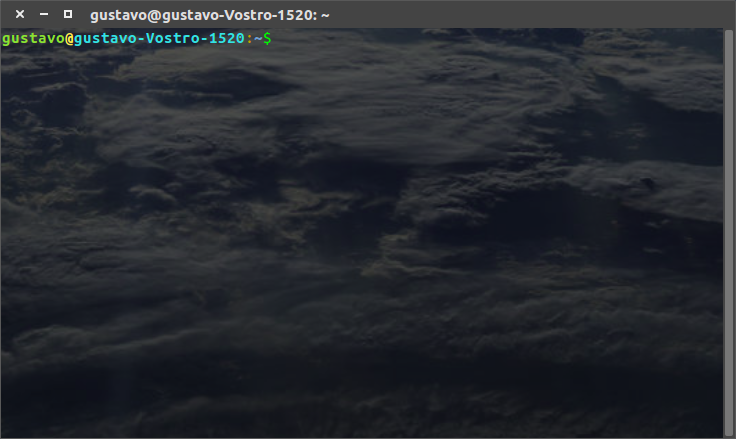
\includegraphics[scale=0.4]{Terminal_01}
	\caption{Pantalla de una terminal en linux.}
\end{figure}
\end{frame}
\begin{frame}
\frametitle{El prompt de la terminal}
En la terminal vemos el llamado \enquote{prompt}, que es el símbolo de dinero  \textasciitilde $\$$
\\
\bigskip
A partir de este momento, linux está en la espera de las instrucciones que ingresemos con el teclado.
\end{frame}
\begin{frame}
\frametitle{Precauciones}
Tengan en cuenta que linux es un sistema operativo diferente, ya que una vez que tecleemos \keys{\return} (la tecla \textbf{Enter}) no se nos pide alguna confirmación, sencillamente se ejecuta la instrucción.
\end{frame}
\begin{frame}
\frametitle{Usar python desde la terminal}
Para usar \python{} desde la terminal, basta con que ingresemos la siguiente instrucción en la terminal:
\begin{center}
\textasciitilde $\$$ \texttt{python} \keys{\return}
\end{center}
\end{frame}
\begin{frame}
\frametitle{Usar python desde la terminal}
\begin{figure}
	\centering
	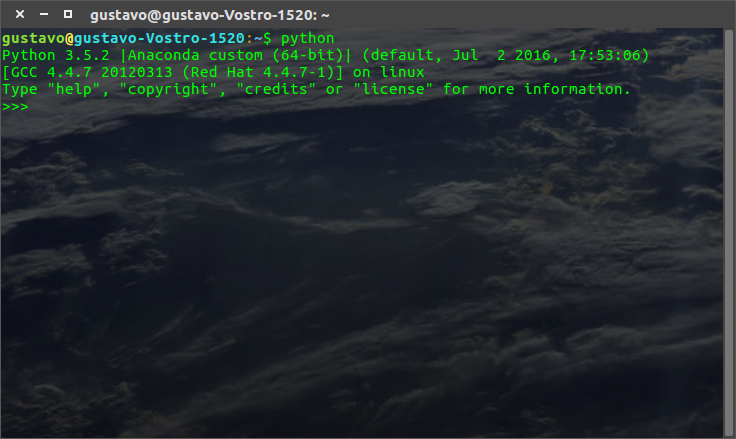
\includegraphics[scale=0.25]{Terminal_02}
	\caption{Vemos cierta información sobre la versión de python instalada en nuestro equipo.}
\end{figure}
\end{frame}
\begin{frame}
\frametitle{El entorno de python en la terminal}
Una vez que ya ingresamos al entorno de \python{} desde la terminal, destacamos el hecho de que el prompt ya cambió: ahora se presenta como $>>>$
\\
\bigskip
Y de nueva cuenta, ahora las instrucciones se deben de escribir en la línea de comandos, pero son instrucciones del lenguaje \python.	
\end{frame}
\begin{frame}
\frametitle{Todo listo para trabajar con \python}
Para ver un saludo en pantalla, escribimos lo siguiente:
\begin{center}
$>>>$ \texttt{print("Hola mundo!")} \keys{\return}
\end{center}
\end{frame}
\begin{frame}
\frametitle{Todo listo para trabajar con \python}
\begin{figure}
	\centering
	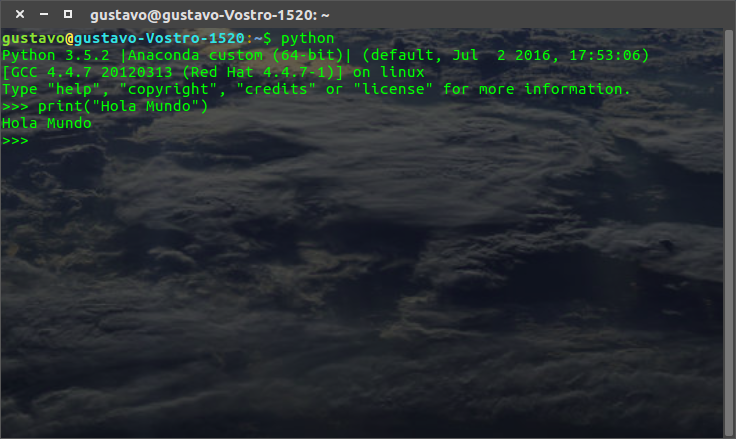
\includegraphics[scale=0.25]{Terminal_03}
	\caption{Obtenemos la respuesta en la siguente línea de la terminal de \python.}
\end{figure}
\end{frame}
\begin{frame}
\frametitle{Salir del entorno de \python{} en la terminal}
Par salir del entorno de python en la terminal de linux, basta con escribir:
\begin{center}
$>>>$ \texttt{exit()} \keys{\return}
\end{center}
\end{frame}
\begin{frame}
\frametitle{Salir del entorno de \python{} en la terminal}
\begin{figure}
	\centering
	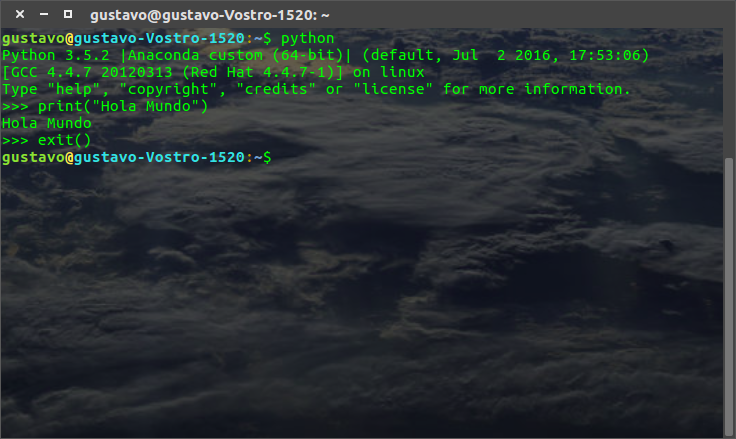
\includegraphics[scale=0.25]{Terminal_04}
	\caption{Regresamos al entorno de linux, revisa el prompt de la terminal.}
\end{figure}
\end{frame}
\section{Anaconda y python}
\frame{\tableofcontents[currentsection, hideothersubsections]}
\subsection{Usando Anaconda}
{
\setbeamercolor{frametitle}{fg=bisque,bg=ao!90!white}
\begin{frame}
\frametitle{Entorno más agradable de trabajo}
El entorno de trabajo para \python{} en la terminal se vuelve en ocasiones muy tedioso, no hay manera de mejorar más allá de la tipografía y fondo de la terminal.
\\
\bigskip
Pero podemos aprovechar al máximo otra herramienta para el curso: \textoazul{\texttt{qtConsole}}, que está integrada en Anaconda\footnote{Revisa la guía de instalación de la suite Anaconda}.
\end{frame}
\begin{frame}
\frametitle{Usaremos ahora qtConsole}
Para trabajar con \textoazul{qtConsole}, con la terminal llamamos a la suite \textoazul{Anaconda}, por lo que escribrimos:
\begin{center}
\textasciitilde $\$$ \texttt{anaconda-navigator} \keys{\return}
\end{center}
\end{frame}
\begin{frame}
\frametitle{Veremos ahora la pantalla de Anaconda}
\begin{figure}
	\centering
	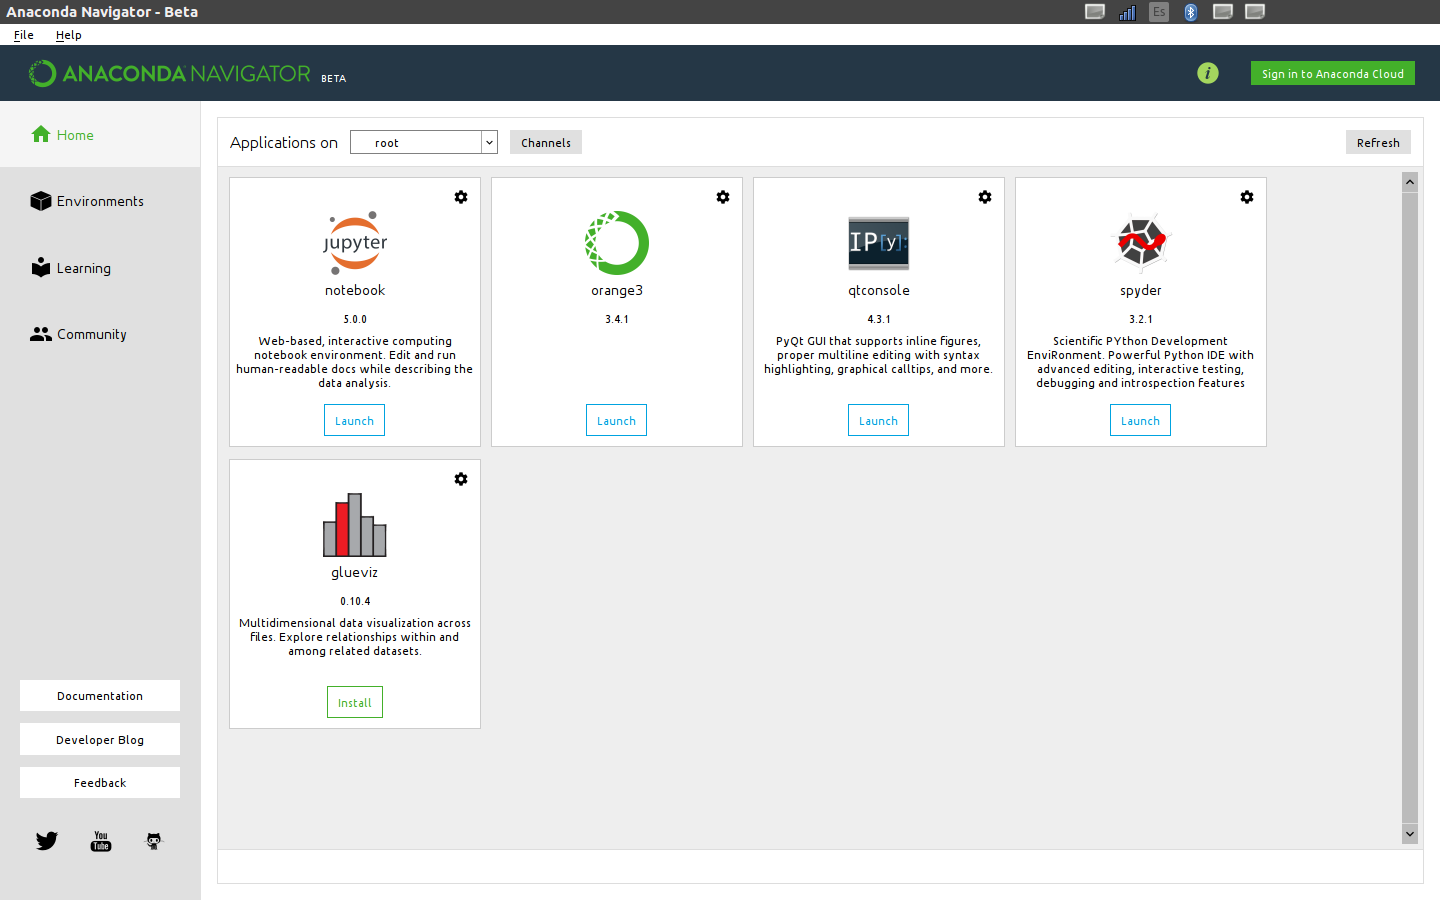
\includegraphics[scale=0.2]{anaconda_01.png}
	%\caption{La suite Anaconda}
\end{figure}
\end{frame}
\begin{frame}
\frametitle{Elegimos qtConsole}
Veremos diferentes programas que están incluidos en la suite, presionamos el botón \textoazul{Launch}, de \textoazul{qtConsole}:
\begin{figure}
	\centering
	
\includegraphics[scale=0.35]{qtConsole_00.png}
	%\caption{Para ejecutar \textoazul{qtConsole}, presionamos \textoazul{Launch}}
\end{figure}
\end{frame}
\begin{frame}
\frametitle{La ventana de qtConsole}
\begin{figure}
	\centering
	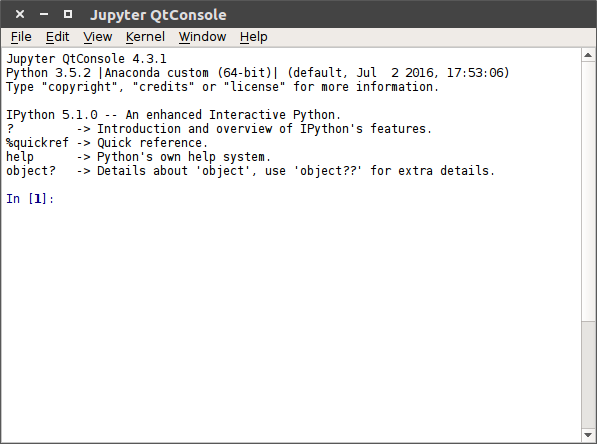
\includegraphics[scale=0.35]{qtConsole_01.png}
	\caption{La ventana de trabajo de qtConsole}
\end{figure}
\end{frame}
\begin{frame}
\frametitle{Personalización de qtConsole}
\begin{figure}
	\centering
	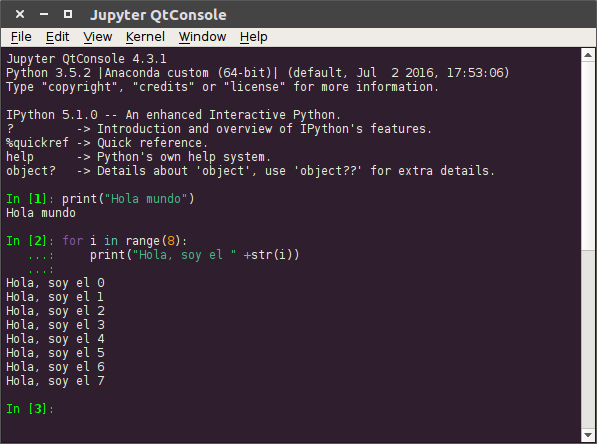
\includegraphics[scale=0.35]{qtConsole_02}
	\caption{Podemos pesonalizar la ventana de trabajo, al seleccionar un estilo de colores y resaltado en el Menú: View $>$ Syntax style}
\end{figure}
\end{frame}
\section{python como una calculadora}
\frame{\tableofcontents[currentsection, hideothersubsections]}
\subsection{Operadores aritméticos}
\begin{frame}
\frametitle{\python{} como calculadora}
Una vez abierta la sesión en \python, podemos aprovechar al máximo este lenguaje: contamos con una calculadora a la mano, sólo hay que ir escribiendo las operaciones en la línea de comandos.
\end{frame}
\setbeamercolor{block title}{bg=red!50,fg=black}
\begin{frame}[fragile]
\frametitle{Algunas operaciones}
Podemos hacer una suma
\\
\bigskip
\textcolor{ao}{\texttt{In[1]: }} \verb|3 + 200| \\
\pause
\textcolor{red}{\texttt{Out[1]: }} \verb|203|
\end{frame}
\begin{frame}[fragile]
\frametitle{Identificador en la línea de comandos}
Nótese que en cada línea tendremos un \enquote{prompt} que nos indica la \emph{entrada}, 
\\
\bigskip
\textcolor{ao}{\texttt{In[1]: }}
\pause
\\
\bigskip
y se le asigna un número consecutivo.
\end{frame}
\begin{frame}[fragile]
\frametitle{Identificador en la línea de comandos}
Dependiendo de la tarea que se ejecute, podemos tener una línea de \emph{salida} con el mismo número
\\
\bigskip
\textcolor{red}{\texttt{Out[1]: }}
\\
\bigskip
\pause
En ciertas tareas, no se presentará esa línea de salida, sino que se mostrará una nueva línea de entrada, con su número consecutivo.
\end{frame}
\begin{frame}[fragile]
\frametitle{Algunas operaciones}
Ahora hagamos una divisón entre enteros
\\
\bigskip
\textcolor{ao}{\texttt{In[2]: }} \verb|30 / 1234| \\
\pause
\textcolor{red}{\texttt{Out[2]: }} \verb|0.024311183144246355|
\end{frame}
\begin{frame}[fragile]
\frametitle{Algunas operaciones}
Una división entre reales
\\
\bigskip
\textcolor{ao}{\texttt{In[3]: }} \verb| 3.0 / 4.0| \\
\pause
\textcolor{red}{\texttt{Out[3]: }} \verb| 0.75|
\end{frame}
\begin{frame}[fragile]
\frametitle{Algunas operaciones}
Una división entera: devuelve el cociente sin decimales
\\
\bigskip
\textcolor{ao}{\texttt{In[4]: }} \verb|30 // 4| \\
\pause
\textcolor{red}{\texttt{Out[4]: }} \verb| 7|
\end{frame}
\begin{frame}[fragile]
\frametitle{Algunas operaciones}
Una división entera: Otro ejemplo de un cociente sin decimales
\\
\bigskip
\textcolor{ao}{\texttt{In[5]: }} \verb|4 // 3| \\
\pause
\textcolor{red}{\texttt{Out[5]: }} \verb| 1|
\end{frame}
\begin{frame}[fragile]
\frametitle{Combinación de operadores artiméticos}
En ocasiones tendremos que realizar en una misma línea de código, varias operaciones artiméticas:
\\
\bigskip
\textcolor{ao}{\texttt{In[6]: }} \verb| 5.0 / 10 * 2 + 5| \\
\pause
\textcolor{red}{\texttt{Out[6]: }} \verb| 6.0|
\pause
\\
\bigskip
\textbf{¿por qué obtenemos este resultado?}
\end{frame}
\begin{frame}[fragile]
\frametitle{Uso de paréntesis}
El resultado cambia cuando agrupamos con paréntesis:
\\
\bigskip
\textcolor{ao}{\texttt{In[7]: }} \verb| 5.0 / (10 * 2 + 5)| \\
\pause
\textcolor{red}{\texttt{Out[7]: }} \verb| 0.2|
\pause
\\
\bigskip
Como podemos ver, el uso de paréntesis en las expresiones tiene una particular importancia sobre el orden en que se evalúan las expresiones.
\end{frame}
\begin{frame}[fragile]
\frametitle{Más operaciones artiméticas}
Potenciación de un número: podemos elevar cualquier número a una potencia en particular
\\
\bigskip
\textcolor{ao}{\texttt{In[8]: }}  \verb| 2 ** 3| \\
\pause
\textcolor{red}{\texttt{Out[8]: }} \verb| 8|
\end{frame}
\begin{frame}[fragile]
\frametitle{Más operaciones artiméticas}
Operador módulo: el operador módulo $\%$ nos devuelve el residuo del cociente:
\\
\bigskip
\textcolor{ao}{\texttt{In[9]: }} \verb| 17 % 3| \\
\pause
\textcolor{red}{\texttt{Out[9]: }} \verb| 2|
\end{frame}
\subsection{Tabla de operadores}
\begin{frame}
\frametitle{Tabla de lo operadores aritméticos}
\begin{table}
\fontsize{12}{12}\selectfont
\begin{tabular}{|c | l | c | c|}
\hline
Operador & Operación & Ejemplo & Resultado \\ \hline
$**$ & Potencia & $2**3$ & $8$ \\ \hline
$*$ & Multiplicación & $7*3$ & $21$ \\ \hline
$/$ & División & $10.5/2$ & $5.25$ \\ \hline
$ //$ & Div. entera & $10.5//2 $ & $5.0$ \\ \hline
$+$ & Suma & $3+4$ & $7$ \\ \hline
$-$ & Resta & $6-8$ & $-2$ \\ \hline
$\%$ & Módulo & $15\%6$ & $3$ \\ \hline
\end{tabular}
\end{table}
\end{frame}
\begin{frame}
\frametitle{Precedencia de los operadores aritméticos}
\setbeamercolor{item projected}{bg=blue!70!black,fg=yellow}
\setbeamertemplate{enumerate items}[circle]
\begin{enumerate}[<+->]
\item Las expresiones contenidas dentro de pares de paréntesis se evalúan primero. 
\item En el caso de expresiones con paréntesis anidados, los operadores en el par de paréntesis más interno se evalúan primero.
\item Las operaciones de exponentes se evalúan después. Si una expresión contiene muchas operaciones de exponentes, los operadores se evalúan de derecha a izquierda.
\end{enumerate}
\end{frame}
\begin{frame}
\frametitle{Precedencia de los operadores aritméticos}
\setbeamercolor{item projected}{bg=blue!70!black,fg=yellow}
\setbeamertemplate{enumerate items}[circle]
\begin{enumerate}[<+->]
\setcounter{enumi}{3}
\item La multiplicación, división y módulo son las siguientes en ser evaluadas. 
\item Si una expresión contiene muchas multiplicaciones, divisiones u operaciones de módulo, los operadores se evaláun de izquierda a derecha.
\end{enumerate}
\end{frame}
\begin{frame}
\frametitle{Precedencia de los operadores aritméticos}
\setbeamercolor{item projected}{bg=blue!70!black,fg=yellow}
\setbeamertemplate{enumerate items}[circle]
\begin{enumerate}[<+->]
\setcounter{enumi}{5}
\item La suma y resta son las operaciones que se evalúan al último. 
\item Si una expresión contiene muchas operaciones de suma y resta, los operadores se evalúan de izquierda a derecha.
\item La suma y resta tienen el mismo nivel de precedencia.
\end{enumerate}
\end{frame}
\section{Operadores relacionales en python}
\frame{\tableofcontents[currentsection, hideothersubsections]}
\subsection{Operadores relacionales}
\begin{frame}
\frametitle{Operadores relacionales}
Cuando se comparan dos (o más expresiones) mediante un operador, el tipo de dato que se devuelve es lógico: \textoazul{\textbf{True}} o \textcolor{red}{\textbf{False}}, que también tienen una representación de tipo numérico:
\begin{itemize}
\item \textoazul{\textbf{True}} = $1$
\item \textcolor{red}{\textbf{False}} = $0$
\end{itemize}
\end{frame}
\begin{frame}[fragile]
\frametitle{Operaciones aritméticas y relacionales}
Podemos extender el manejo con \python, al combinar las operaciones aritméticas y relacionales, nótese que siempre tendremos como respuesta un valor booleano:
\\
\bigskip
\textcolor{ao}{\texttt{In[10]: }} \verb| 1 + 2 > 7 - 3| \\
\pause
\textcolor{red}{\texttt{Out[10]: }} \verb| False|
\end{frame}
\begin{frame}[fragile]
\frametitle{Operaciones aritméticas y relacionales}
Otro ejemplo en donde ahora tenemos dos expresiones relacionales:
\\
\bigskip
\textcolor{ao}{\texttt{In[11]: }} \verb| 1 < 2 < 3| \\
\pause
\textcolor{red}{\texttt{Out[11]: }} \verb| True|
\end{frame}
\begin{frame}[fragile]
\frametitle{El operador de comparación de igualdad}
El doble signo igual ($==$) es el operador de igualdad, a diferencia del operador $=$ que es el operador de asignación.
\\
\bigskip
\textcolor{ao}{\texttt{In[12]: }} \verb| 1 > 2 == 2 < 3| \\
\pause
\textcolor{red}{\texttt{In[12]: }} \verb| False|
\end{frame}
\begin{frame}[fragile]
\frametitle{Combinación de expresiones}
\textcolor{ao}{\texttt{In[13]: }} \verb| 3 > 4 < 5| \\
\pause
\textcolor{red}{\texttt{In[13]: }} \verb| False|
\\
\bigskip
\pause
\textcolor{ao}{\texttt{In[14]: }} \verb| 1.0 / 3 < 0.3333| \\
\pause
\textcolor{red}{\texttt{In[14]: }} \verb| False|
\\
\bigskip
\pause
\textcolor{ao}{\texttt{In[15]: }} \verb| 5.0 / 3 >= 11 /7.0| \\
\pause
\textcolor{red}{\texttt{In[15]: }} \verb| True|
\\
\bigskip
Las expresiones se pueden complicar cada vez más, por lo que hay que mantener atención al momento de escribirlas.
\end{frame}
\begin{frame}
\frametitle{Tabla de operadores relacionales}
\begin{table}
\fontsize{12}{12}\selectfont
\begin{tabular}{| c | l | c | c |}
\hline
Operador & Operación & Ejemplo & Resultado\\ \hline
$==$ & Igual a & $4==5$ & \textcolor{red}{\texttt{False}} \\ \hline
$!=$ & Diferente & $2!=3$ & \textoazul{\texttt{True}} \\ \hline
$<$ & Menor que & $ 10<4$  & \textcolor{red}{\texttt{False}} \\ \hline
$>$ & Mayor que & $5>-4$ & \textoazul{\texttt{True}} \\ \hline
$<=$ & Menor o igual & $7<=7$ & \textoazul{\texttt{True}} \\ \hline
$>=$ & Mayor o igual & $3.5 >= 10$ & \textcolor{red}{\texttt{False}} \\ \hline
\end{tabular}
\end{table}
\end{frame}
\begin{frame}[fragile]
\frametitle{Posibles errores al introducir valores/operaciones}
Será muy común al inicio encontrar errores cuando se teclean las instrucciones en el código, por lo que hay que tomar en cuenta los avisos que nos devuelve \python:
\\
\bigskip
\pause
\textcolor{ao}{\texttt{In[16]: }} \verb| 5 + |
\\
\pause
\verb| File "<stdin>", line 1| \\
\verb|      5 +  | \\
\verb|         ^| \\
\textcolor{red}{\texttt{SyntaxError:}}\verb| invalid syntax|
\end{frame}
\begin{frame}[fragile]
\frametitle{Posibles errores al introducir valores/operaciones}
\textcolor{ao}{\texttt{In[17]: }} \verb| 42 + 5 + * 2 |
\\
\pause
\verb| File "<stdin>", line 1| \\
\verb|   42 + 5 + * 2 | \\
\verb|            ^| \\
\textcolor{red}{\texttt{SyntaxError:}}\verb| invalid syntax|
\end{frame}
\section{Operadores booleanos en python}
\frame{\tableofcontents[currentsection, hideothersubsections]}
\subsection{Operadores booleanos}
\begin{frame}
\frametitle{Operadores booleanos}
Existen en \python{} tres operadores booleanos:
\setbeamercolor{item projected}{bg=blue!70!black,fg=yellow}
\setbeamertemplate{enumerate items}[circle]
\begin{enumerate}[<+->]
\item \azulfuerte{and}
\item \azulfuerte{or}
\item \azulfuerte{not}
\end{enumerate}
\pause
Estos operadores comparan valores booleanos, el resultado de ésta comparación se expresa en un valor booleano.
\end{frame}
\begin{frame}[fragile]
\frametitle{El operador booleano \texttt{and}}
Cuando comparamos dos expresiones con el operador booleano \azulfuerte{and}, tendremos de respuesta un valor \textoazul{True}, siempre y cuando ambas expresiones sean verdaderas:
\\
\bigskip
\pause
\textcolor{ao}{\texttt{In[18]: }} \verb| (4 < 5) and (5 < 6)| \\
\pause
\textcolor{red}{\texttt{Out[18]: }} \verb| True|
\end{frame}
\begin{frame}[fragile]
\frametitle{El operador booleano \texttt{and}}
En caso de que una de las expresiones sea \textoazul{False} (incluso las dos expresiones), al momento de compararlas con el operador booleano \azulfuerte{and}, el resultado que se devuelve es \azulfuerte{False}:
\\
\bigskip
\pause
\textcolor{ao}{\texttt{In[19]: }} \verb| (4 < 5) and (9 < 6)| \\
\pause
\textcolor{red}{\texttt{Out[19]: }} \verb| False|
\end{frame}
\begin{frame}[fragile]
\frametitle{El operador booleano \texttt{or}}
El operador booleano \azulfuerte{or} devuelve un valor \textoazul{True}, cuando una de las expresiones es verdadera (incluso ambas):
\\
\bigskip
\pause
\textcolor{ao}{\texttt{In[20]: }} \verb| (1==2) or (2 == 2)| \\
\pause
\textcolor{red}{\texttt{Out[20]: }} \verb| True|
\end{frame}
\begin{frame}[fragile]
\frametitle{El operador booleano \texttt{or}}
Si las expresiones que se comparan con el operador booleano \azulfuerte{or} son ambas falsas, se tendrá como respuesta un valor \textoazul{False}:
\\
\bigskip
\pause
\textcolor{ao}{\texttt{In[21]: }} \verb| (1 > 2) or (8 == 2)| \\
\pause
\textcolor{red}{\texttt{Out[21]: }} \verb| False|
\end{frame}
\begin{frame}[fragile]
\frametitle{El operador booleano \texttt{not}}
El operador booleano \azulfuerte{not} \enquote{niega} (invierte) el valor booleano de la expresión que evalúa:
\\
\bigskip
\pause
\textcolor{ao}{\texttt{In[22]: }} \verb| not(True)| \\
\pause
\textcolor{red}{\texttt{Out[22]: }} \verb| False|
\end{frame}
\begin{frame}[fragile]
\frametitle{El operador booleano \texttt{not}}
Podemos ocupar una expresión más elaborada en la que anticipamos el resultado y entonces se ocupa el operador \azulfuerte{not}, para negar el resultado:
\\
\bigskip
\pause
\textcolor{ao}{\texttt{In[23]: }} \verb| ((2 + 2) == 4) and (not ((2 + 2) == 5)))| \\
\pause
\textcolor{red}{\texttt{Out[23]: }} \verb| True|
\end{frame}
% \begin{frame}
% \frametitle{Tabla de resumen}
% Como se verá en la siguiente tabla, se necesita una condición particular para que el valor que devuelva la comparación, sea \textcolor{red}{\texttt{False}}.
% \begin{table}
% \fontsize{12}{12}\selectfont
% \begin{tabular}{| c | l | c | c |}
% \hline
% Operador & Operación & Ejemplo & Resultado \\ \hline
% \texttt{and} & Conjunción & \textcolor{red}{False} and \textoazul{True} & \textcolor{red}{False} \\ \hline
% \texttt{or} & Disyunción & \textcolor{red}{False} or \textoazul{True}  &
% \textoazul{True} \\ \hline
% \texttt{not} & Negación & \texttt{not} \textoazul{True} & \textcolor{red}{False} \\ \hline
% \end{tabular}
% \end{table}
% \end{frame}
\begin{frame}
\frametitle{Tabla de verdad de los operadores booleanos}
Se utilizan dos expresiones booleanas \textbf{A} y \textbf{B}, y se comparan con los operadores booleanos de \python{}:
\begin{table}
\begin{tabular}{| c | c | c | c | c |}
\hline
A & B & A \texttt{and} B & A \texttt{or} B & \texttt{not} A\\ \hline
\textoazul{True} & \textoazul{True} & \textoazul{True} & \textoazul{True} & \textcolor{red}{False}\\ \hline
\textoazul{True} & \textcolor{red}{False} & \textcolor{red}{False} & \textoazul{True} & \textcolor{red}{False} \\ \hline
\textcolor{red}{False} & \textoazul{True} & \textcolor{red}{False} & \textoazul{True} & \textoazul{True}\\ \hline
\textcolor{red}{False} & \textcolor{red}{False} & \textcolor{red}{False} & \textcolor{red}{False} & \textoazul{True} \\ \hline
\end{tabular}
\end{table}
\end{frame}
\section{Las variables en \python}
\frame{\tableofcontents[currentsection, hideothersubsections]}
\subsection{Tipos de variables}
\begin{frame}
\frametitle{Tipos de variables}
Las variables en \python{} sólo son ubicaciones de memoria reservadas para almacenar valores.
\\
\bigskip
Esto significa que cuando se crea una variable, se reserva un poco de espacio disponible en la memoria.
\end{frame}
\begin{frame}
\frametitle{Tipos de variables}
Basándose en el tipo de datos de una variable, el intérprete asigna memoria y decide qué se puede almacenar en la memoria reservada.
\\
\bigskip
Presentamos tres tipos de datos:
\setbeamercolor{item projected}{bg=blue!70!black,fg=yellow}
\setbeamertemplate{enumerate items}[circle]
\begin{enumerate}[<+->]
\item Tipo \textbf{Entero}: números con signo, sin decimales.
\item Tipo \textbf{Punto flotante}: números con decimales.
\item Tipo \textbf{Cadenas}: caracteres.
\end{enumerate}
\end{frame}
\begin{frame}
\frametitle{Asignando valores a variables}
Las variables en \python{} no necesitan una declaración explícita para reservar el espacio en memoria. La declaración ocurre automáticamente cuando se asigna un valor a una variable.
\\
\bigskip
\pause
\emph{El signo igual (=) se utiliza para asignar valores a las variables}.
\end{frame}
\begin{frame}[fragile]
\frametitle{Asignando valores a variables}
\textcolor{blue}{temperatura} = \textcolor{brown}{37.8}
\\
\bigskip
El término a la izquierda del operador $=$ es el \textoazul{\emph{nombre de la variable}} y el término a la derecha del operador $=$ es el \textcolor{brown}{\emph{valor almacenado}} en la variable.
\end{frame}
\begin{frame}[fragile]
\frametitle{Ejemplos de asignación de variables}
A continuación se asigna un valor a tres tipos de variables\footnote{Nótese que no se genera una línea de salida en qtConsole.}: entera, de punto flotante y de cadena:
\\
\bigskip
\pause
\textcolor{ao}{\texttt{In[24]: }} \verb| contador = 100| \\ \pause
\textcolor{ao}{\texttt{In[25]: }} \verb| distancia = 1000.50| \\ \pause
\textcolor{ao}{\texttt{In[26]: }} \verb| nombre = "Goyo"|
\end{frame}
\begin{frame}[fragile]
\frametitle{Visualización del contenido de las variables}
Para \enquote{ver} el contenido de una variable, escribimos el nombre de la misma, al presionar la tecla Enter, se devuelve el valor asignado:
\\
\bigskip
\pause
\textcolor{ao}{\texttt{In[27]: }} \verb| contador| \\
\pause
\textcolor{red}{\texttt{Out[27]: }} \verb| 100| \\
\pause
\textcolor{ao}{\texttt{In[28]: }} \verb| distancia| \\
\pause
\textcolor{red}{\texttt{Out[28]: }} \verb| 1000.50| \\
\pause
\textcolor{ao}{\texttt{In[29]: }} \verb| nombre| \\
\pause
\textcolor{red}{\texttt{Out[29]: }} \verb| Goyo|
\end{frame}
\begin{frame}[fragile]
\frametitle{Asignación múltiple de valores}
En \python{} podemos asignar un valor único a varias variables de manera simultánea:
\\
\bigskip
\pause
\textcolor{ao}{\texttt{In[30]: }} \verb| A = b = c = 1 | \\
\pause
\textcolor{ao}{\texttt{In[31]: }} \verb| A | \\
\pause
\textcolor{red}{\texttt{Out[31]: }} \verb| 1 | \\
\pause
\textcolor{ao}{\texttt{In[32]: }} \verb| b | \\
\pause
\textcolor{red}{\texttt{Out[32]: }} \verb| 1 | \\
\pause
\textcolor{ao}{\texttt{In[33]: }} \verb| c | \\
\pause
\textcolor{red}{\texttt{Out[33]: }} \verb| 1 |
\end{frame}
\begin{frame}[fragile]
\frametitle{Asignación múltiple a varias variables}
También podemos asignar varios valores a varias variables de manera simultánea, separando con una coma tanto a las variables como a los valores:
\end{frame}
\begin{frame}[fragile]
\frametitle{Asignación múltiple a varias variables}
\textcolor{ao}{\texttt{In[34]: }} \verb| usuario, folio, temp = "Poncho", 100, 37.3 | \\
\pause
\textcolor{ao}{\texttt{In[35]: }} \verb| usuario | \\
\pause
\textcolor{red}{\texttt{Out[35]: }} \verb| 'Poncho'| \\
\pause
\textcolor{ao}{\texttt{In[36]: }} \verb| folio | \\
\pause
\textcolor{red}{\texttt{Out[36]: }} \verb| 100| \\
\pause
\textcolor{ao}{\texttt{In[37]: }} \verb| temp| \\
\pause
\textcolor{red}{\texttt{Out[37]: }} \verb| 37.3|
\end{frame}
\section{Tipos de Datos Estándar}
\frame[allowframebreaks]{\tableofcontents[currentsection, hideothersubsections]}
\subsection{Los tipos de datos en \python}
\begin{frame}
\frametitle{Tipos de datos}
Los datos almacenados en la memoria pueden ser de varios tipos. Por ejemplo, la edad de una persona se almacena como un valor numérico y su dirección se almacena como caracteres alfanuméricos.
\\
\bigskip
En \python{} se cuenta con varios tipos de datos estándar que se utilizan para definir las operaciones posibles entre ellos y el método de almacenamiento para cada uno de ellos.
\end{frame}
\begin{frame}
\frametitle{Tipos de datos}
Los tipos de datos que se utilizan en \python{} son cinco:
\setbeamercolor{item projected}{bg=blue!70!black,fg=yellow}
\setbeamertemplate{enumerate items}[circle]
\begin{enumerate}[<+->]
\item Números.
\item Cadena.
\item Lista.
\item Tupla.
\item Diccionario.
\end{enumerate}
\end{frame}
\begin{frame}
\frametitle{Números}
Los tipos de datos numéricos almacenan valores numéricos.
\\
\bigskip
Los objetos numéricos se crean cuando se les asigna un valor.
\end{frame}
\begin{frame}[fragile]
\frametitle{Declaración en variables}
\textcolor{ao}{\texttt{In[38]: }} \verb| var1 = var2 = 10| \\
\pause
\textcolor{ao}{\texttt{In[39]: }} \verb| var1| \\
\pause
\textcolor{red}{\texttt{Out[39]: }} \verb| 10| \\
\pause
\textcolor{ao}{\texttt{In[40]: }} \verb| var2| \\
\pause
\textcolor{red}{\texttt{Out[40]: }} \verb| 10|
\end{frame}
\begin{frame}
\frametitle{Eliminando variables en \python}
También se puede eliminar la referencia a una variable numérica utilizando la sentencia \azulfuerte{del}
\\
\bigskip
La sintaxis de la sentencia \texttt{del} es:
\\
\bigskip
\texttt{del var1 [, var2 [, var3 [...., varN]]]]}
\\
\bigskip
los corchetes indican que hay parámetros que son opcionales.
\end{frame}
\begin{frame}[fragile]
\frametitle{Eliminando variables en \python}
Se puede eliminar una sola variable o varias utilizando la sentencia \azulfuerte{del}
\\
\bigskip
Por ejemplo, la variable \textoazul{var1} que ya teníamos referenciada previamente:
\\
\bigskip
\textcolor{ao}{\texttt{In[41]: }} \verb| del var1|
\end{frame}
\begin{frame}[fragile]
\frametitle{Eliminando variables en \python{arg}}
Si desde la terminal hacemos referencia a la variable eliminada, tendremos un mensaje como el siguiente:
\textcolor{ao}{\texttt{In[42]: }} \verb| var1|
\begin{verbatim}
NameError   Traceback (most recent call last)
<stdin> in <module>
----> 1 var1

NameError: name 'var1' is not defined
\end{verbatim}
La variable ya no existe y no podemos recuperarla.
\end{frame}
\subsection{Tipos de datos numéricos}
\begin{frame}
\frametitle{Tipos de datos numéricos}
En \python{} se soportan tres tipos numéricos diferentes:
\setbeamercolor{item projected}{bg=blue!70!black,fg=yellow}
\setbeamertemplate{enumerate items}[circle]
\begin{enumerate}[<+->]
\item Int (enteros con signo)
\item De punto flotante (valores reales con decimales)
\item Complejos (números complejos)
\end{enumerate}
\end{frame}
\begin{frame}
\frametitle{Números enteros}
Los números enteros son aquellos que no tienen decimales, tanto positivos como negativos (además del cero). En \python{} se representan mediante el tipo \texttt{int} (de integer, entero).
\\
\bigskip
Todos los números enteros en \python 3 se representan como enteros largos.
\end{frame}
\begin{frame}
\frametitle{Números flotantes o reales}
Los números reales son los que tienen decimales. En \python{} se expresan mediante el tipo \texttt{float}.
\\
\bigskip
En \python{} se implementa su tipo float utilizando 64 bits, en concreto se sigue el estándar IEEE 754\footnote{En el Tema 1, ampliaremos esta información}: 1 bit para el signo, 11 para el exponente, y 52 para la mantisa.
\end{frame}
\begin{frame}
\frametitle{Números complejos}
Un número complejo consiste en un par ordenado de números reales de coma flotante denotados por
\[ x + y \: j\]
donde $x$ e $y$ son números reales, $y \: j$ es la unidad imaginaria.
\end{frame}
\begin{frame}
\frametitle{Ejemplos de tipos de datos numéricos}
\begin{table}
\begin{tabular}{| c | c | c |}
\hline
\texttt{int} & \texttt{float} & \texttt{complex} \\ \hline
$10$ & $0.0$ & $3.14 \: j$ \\ \hline
$100$ & $15.20$ & $45.j$ \\ \hline
$100$ & $-15.20$ & $23.15+7.5j$ \\ \hline
$080$ & $32.3+e18$ & $0.876j$ \\ \hline
$-0490$ & $-90.$ & $-0.645+0j$ \\ \hline
$-0x260$ & $-32.54e100$ & $3e+26j$ \\ \hline
$0x69$ & $70.2-E12$ & $4.53e-7j$ \\ \hline
\end{tabular}
\end{table}    
\end{frame}
\subsection{Cadenas}
\begin{frame}
\frametitle{Cadenas en python}
Las cadenas en \python{} se identifican como un conjunto contiguo de caracteres representados en las comillas.
\\
\bigskip
Con \python{} se permite cualquier par de 'comillas simples' o comillas \enquote{dobles}.
\end{frame}
\begin{frame}
\frametitle{Operación con cadenas}
Los subconjuntos de cadenas pueden ser tomados usando el operador de corte $[ \quad ]$ y $[:]$ con los índices comenzando en $0$ al inicio de la cadena hasta llegar a $-1$ al final de la misma.
\pause
El signo más $+$ es el operador de concatenación de cadenas y el asterisco $*$ es el operador de repetición.
\end{frame}
\begin{frame}[fragile]
\frametitle{Ejemplo de una variable de tipo cadena}
Declaremos una variable con un tipo de dato cadena:
\\
\bigskip
\textcolor{ao}{\texttt{In[43]: }} \verb| facultad = "Ciencias"|
\end{frame}
\begin{frame}
\frametitle{Manipulando la variable de tipo cadena}
Es necesario conocer la manera en la que se almacena una variable de tipo cadena:
\begin{figure}
\includestandalone{Figuras/variablecadena01}
\end{figure}
cada caracter se almacena en un espacio que se identifica mediante un índice, en \python{} los índices comienzan en cero.

% >>> cadena = 'Hola Mundo!'

% >>> print (cadena)
% >>> print (cadena[0])
% >>> print (cadena[2:5])     
% >>> print (cadena[2:])
% >>> print (cadena * 2)
% >>> print (cadena + "PUMAS")
% \end{verbatim}
\end{frame}
\begin{frame}[fragile]
\frametitle{Recuperando el contenido de la cadena}
Con el debido manejo de los índices podemos recuperar el contenido de la variable de tipo cadena, para ello recurrimos al manejo de los índices con corchetes:
\\
\bigskip
\pause
\textcolor{ao}{\texttt{In[44]: }} \verb| facultad[0]|
\\
\pause
\textcolor{red}{\texttt{Out[44]: }} \verb| 'C'|
\\
\medskip
Como vemos, se recupera el primer caracter de la variable.
\end{frame}
\begin{frame}[fragile]
\frametitle{Recuperando el contenido de la cadena}
\begin{figure}
	 \includestandalone{Figuras/variablecadena02}
\end{figure}
\end{frame}
\begin{frame}[fragile]
\frametitle{Recuperando el contenido de la cadena}
El manejo de los índices en \python{} es muy versátil, al utilizar un número negativo podemos recorrer en sentido inverso el contenido de la variable de cadena, por ejemplo:
\\
\bigskip
\pause
\textcolor{ao}{\texttt{In[45]: }} \verb| facultad[-1]|
\\
\pause
\textcolor{red}{\texttt{Out[45]: }} \verb| 's'|
\end{frame}
\begin{frame}[fragile]
\frametitle{Recuperando el contenido de la cadena}
En sentido inverso, los índices en \python{} inician en $-1$:
\begin{figure}
		\includestandalone{Figuras/variablecadena03}
\end{figure}
\end{frame}
\begin{frame}[fragile]
\frametitle{Recuperando el contenido con slicing}
El término \emph{slicing} hace referencia a un \enquote{rebanado o corte} en una cadena, que es una seleción de la misma, para ello se utilizan los dos puntos dentro del corchete, teniendo las distintas opciones:
\end{frame}
\begin{frame}[fragile]
\frametitle{Recuperando el contenido con slicing}
Recupera el contenido desde \emph{inicio} hasta \emph{fin - 1:}
\\
\bigskip
\verb|cadena[inicio:fin]|
\\
\bigskip
\pause
Recupera el contenido desde \emph{inicio} hasta el resto de la cadena
\\
\bigskip
\verb|cadena[inicio:]|
\end{frame}
\begin{frame}[fragile]
\frametitle{Recuperando el contenido con slicing}
Recupera el contenido desde el inicio hasta \emph{fin - 1:}
\\
\bigskip
\verb|cadena[:fin]|
\\
\bigskip
\pause
Recupera una copia de toda la cadena
\\
\bigskip
\verb|cadena[:]|
\end{frame}
\begin{frame}[fragile]
\frametitle{Ejemplos con el uso del slicing en cadenas}
\textcolor{ao}{\texttt{In[46]: }} \verb| facultad[2:4]|
\\
\pause
\textcolor{red}{\texttt{Out[46]: }} \verb| 'en'|
\\
\bigskip
\pause
\textcolor{ao}{\texttt{In[47]: }} \verb| facultad[2:]|
\\
\pause
\textcolor{red}{\texttt{Out[47]: }} \verb| 'encias'|
\pause
\\
\bigskip
\pause
\textcolor{ao}{\texttt{In[48]: }} \verb| facultad[6:8]|
\\
\pause
\textcolor{red}{\texttt{Out[48]: }} \verb| 'as'|
\end{frame}
\begin{frame}[fragile]
\frametitle{Representación de los índices en el slicing}
Vemos que al usar el \emph{slicing}, algo pasa al momento de asignar los índices, y no recupera propiamente lo que pedimos devuelta, veamos en el siguiente diagrama los índices del contenido de la variable y los índices del \emph{slicing}:
\end{frame}
\begin{frame}[fragile]
\frametitle{Índices de contenido y de slicing}
\begin{figure}
	\includestandalone[scale=0.8]{Figuras/variablecadena05}
\end{figure}
Como vemos, cuando usamos el \emph{slicing} los índices cambian a una posición, no al contenido de la cadena.
\end{frame}
\begin{frame}[fragile]
\frametitle{Operador de repetición}
Cuando tenemos una cadena, es posible repetir un determinado número de veces la misma, para ello se utiliza el operador de repetición $*$:
\\
\bigskip
\pause
\textcolor{ao}{\texttt{In[49]: }} \verb| facultad*2|
\\
\pause
\textcolor{red}{\texttt{Out[49]: }} \verb| 'CienciasCiencias'|
\end{frame}
\begin{frame}[fragile]
\frametitle{Operador de concatenación}
Las variables de tipo cadena se pueden concatenar, es decir, se pueden unir mediante el operador $+$:
\\
\bigskip
\pause
\textcolor{ao}{\texttt{In[50]: }} \verb| Dependencia = 'Facultad de '|
\\
\pause
\textcolor{ao}{\texttt{In[51]: }} \verb| Dependencia + facultad|
\\
\pause
\textcolor{red}{\texttt{Out[51]: }} \verb| 'Facultad de Ciencias'|
\end{frame}
\subsection{Listas}
\begin{frame}
\frametitle{Las listas en \python}
Las listas son el tipo de dato más versátil de los datos compuestos de \python.
\\
\bigskip
Una lista contiene elementos separados por comas y entre corchetes $[ \quad ]$.
\end{frame}
\begin{frame}
\frametitle{Las listas en \python}
En cierta medida, las listas son similares a los arreglos (arrays) en el lenguaje C.
\\
\bigskip
Una de las diferencias entre ellos, es que todos los elementos pertenecientes a una lista pueden ser de tipo de datos diferente.
\end{frame}
\begin{frame}
\frametitle{Las listas en \python}
Los valores almacenados en una lista se pueden acceder utilizando el operador de división $[ \: ]$ y $[:]$ con índices que empiezan en $0$ al principio de la lista y opera hasta el final con $-1$.
\\
\bigskip
El signo más $+$ es el operador de concatenación de lista y el asterisco $*$ es el operador de repetición.
\end{frame}
\begin{frame}[fragile]
\frametitle{Ejemplos con listas}
%\fontsize{12}{12}\selectfont
Para introducir una lista, abrimos corchetes y separamos mediante comas los elementos de la misma:
\\
\pause
\textcolor{ao}{\texttt{In[52]: }} \verb| lista1 = ['abcd', 786, 2.23, 'salmon', 70.2]|
\\
\textcolor{ao}{\texttt{In[53]: }} \verb| lista2 = [ 123, 'pizza']|
\end{frame}
\begin{frame}[fragile]
\frametitle{Operaciones con las listas}
Al igual que con las variables, podemos visualizar el contenido de una lista, al indicarla en la línea de comandos:
\\
\bigskip
\textcolor{ao}{\texttt{In[54]: }} \verb| lista1|
\\
\pause
\textcolor{red}{\texttt{Out[54]: }} \verb| ['abcd', 786, 2.23, 'salmon', 70.2]|
\end{frame}
\begin{frame}[fragile]
\frametitle{Operaciones con las listas 2}
Como en una variable de tipo cadena, el contenido de las listas se realiza con índices: tanto de contenido como de \emph{slicing}:
\\
\bigskip
\textcolor{ao}{\texttt{In[55]: }} \verb| lista1[2:]|
\\
\pause
\textcolor{red}{\texttt{Out[55]: }} \verb| [2.23, 'salmon', 70.2]|
\end{frame}
\begin{frame}[fragile]
\frametitle{Operaciones con las listas 2}
\textcolor{ao}{\texttt{In[56]: }} \verb| lista1[-1]|
\\
\pause
\textcolor{red}{\texttt{Out[56]: }} \verb| [70.2]|
\\
\bigskip
\pause
\textcolor{ao}{\texttt{In[57]: }} \verb| lista1[2:4]|
\\
\pause
\textcolor{red}{\texttt{Out[57]: }} \verb| [2.23, 'salmon']|
\end{frame}
\begin{frame}[fragile]
\frametitle{Operaciones con las listas 2}
También se ocupan las operaciones de concatenación y repetición en las listas:
\\
\bigskip
\textcolor{ao}{\texttt{In[58]: }} \verb| lista1 + lista2|
\\
\pause
\begingroup
\fontsize{13}{13}\selectfont
\textcolor{red}{\texttt{Out[58]: }} \verb| ['abcd', 786, 2.23, 'salmon', 70.2, 123, 'pizza']|
\endgroup
\\
\bigskip
\pause
\textcolor{ao}{\texttt{In[59]: }} \verb| lista2*2|
\\
\pause
\textcolor{red}{\texttt{Out[59]: }} \verb| [123, 'pizza', 123, 'pizza']|
\end{frame}
\begin{frame}[fragile]
\frametitle{Agregar elementos a una lista}
Las listas en \python{} son los únicos objetos en los que podemos agregar nuevos elementos, para ello hay que utilizar la instrucción \textoazul{append}:
\\
\bigskip
\textcolor{ao}{\texttt{In[60]: }} \verb| lista1.append(654.321)|
\\
\pause
\textcolor{ao}{\texttt{In[61]: }} \verb|  lista1|
\\
\pause
\textcolor{red}{\texttt{Out[61]: }} \verb| ['abcd', 786, 2.23, 'salmon', 70.2, 654.321]|
\end{frame}
\begin{frame}[fragile]
\frametitle{Reemplazo de un elemento de la lista}
Con una lista en \python{} se puede reemplazar el contenido específico de un elemento, haciendo referencia al índice en particular:
\\
\bigskip
\textcolor{ao}{\texttt{In[62]: }} \verb|  lista2[1] = 'coordenada'|
\\
\pause
\textcolor{ao}{\texttt{In[63]: }} \verb|  lista2|
\\
\pause
\textcolor{red}{\texttt{Out[63]: }} \verb| [123, 'coordenada']|
\end{frame}
\begin{frame}[fragile]
\frametitle{Característica de las listas}
Las listas son un tipo de objeto en \python{} que permite que dentro de la misma, pueda contener a su vez, otra lista:
\\
\bigskip
\textcolor{ao}{\texttt{In[64]: }} \verb|  lista1.append(lista2)|
\\
\pause
\textcolor{ao}{\texttt{In[65]: }} \verb|  lista1|
\\
\pause
\textcolor{red}{\texttt{Out[65]: }}  
\begin{lstlisting}
['abcd', 786, 2.23, 'salmon', 70.2, 654.321, [123, 'coordenada']]
\end{lstlisting}
\end{frame}
\subsection{Tuplas}
\begin{frame}
\frametitle{Las tuplas en \python}
Una tupla es otro tipo de datos de secuencia que es similar a la lista.
\\
\bigskip
Una tupla consiste en un grupo de valores separados por comas, identificamos a una tupla por que ésta usa paréntesis $( \quad )$.
\end{frame}
\begin{frame}
\frametitle{Característica de las tuplas}
Las principales características de las tuplas son:
\setbeamercolor{item projected}{bg=blue!70!black,fg=yellow}
\setbeamertemplate{enumerate items}[circle]
\begin{enumerate}[<+->]
\item Los elementos de las tuplas no pueden modificarse.
\item No es posible agregar nuevos elementos a un tupla.
\item Identificamos lo que una tupla contiene mediante índices: tanto de contenido como de \emph{slicing}.
\end{enumerate}
\pause
Las tuplas pueden ser consideradas como listas de sólo lectura.
\end{frame}
\begin{frame}[fragile]
\frametitle{Ejemplos con tuplas}
\textcolor{ao}{\texttt{In[66]: }} \verb|  tupla1 = ('abcd', 786, 2.23, 'arena', 70.2)|
\\
\pause
\textcolor{ao}{\texttt{In[67]: }} \verb|  tupla2 = (3.14, 'playa')|
\\
\bigskip
\pause
\textcolor{ao}{\texttt{In[68]: }} \verb| tupla1|
\\
\textcolor{red}{\texttt{Out[68]: }} \verb| ('abcd', 786, 2.23, 'arena', 70.2)|
\end{frame}

\begin{frame}[fragile]
\frametitle{Operación con tuplas}
Podemos seleccionar los elementos de la tupla mediante el uso de índices de contenido
\\
\bigskip
\textcolor{ao}{\texttt{In[69]: }} \verb| tupla1[0]|
\\
\pause
\textcolor{red}{\texttt{Out[69]: }} \verb| 'abcd'|
\\
\bigskip
\pause
Así como usando índices de selección:
\\
\bigskip
\textcolor{ao}{\texttt{In[70]: }} \verb| tupla1[1:3]|
\\
\pause
\textcolor{red}{\texttt{Out[70]: }} \verb| (7.86, 2.23)|
\end{frame}
\begin{frame}[fragile]
\frametitle{Errores con el manejo de tuplas}
Si queremos modificar el contenido de una tupla, obtendremos un mensaje de error
\\
\bigskip
\textcolor{ao}{\texttt{In[71]: }} \verb| tupla1[2] = 'hola'|
\\
\pause
\textcolor{red}{\texttt{Out[71]: }} 
\begingroup
\fontsize{12}{12}\selectfont
\begin{verbatim}
TypeError     Traceback (most recent call last)

<stdin> in <module>()
----> 1 tupla1[2] = 'hola'

TypeError: 'tuple' object does not support
 item assignment
\end{verbatim}
\endgroup
\end{frame}
\begin{frame}[fragile]
\frametitle{Errores con el manejo de tuplas}
Si queremos agregar un elemento a la tupla, obtendremos un mensaje de error
\\
\bigskip
\textcolor{ao}{\texttt{In[72]: }} \verb| tupla1.append(100.56)|
\\
\pause
\textcolor{red}{\texttt{Out[72]: }} 
\begingroup
\fontsize{12}{12}\selectfont
\begin{verbatim}
TypeError     Traceback (most recent call last)

<stdin> in <module>()
----> 1 tupla1.append(100.56)

AttributeError: 'tuple' object has no 
  attribute 'append'
\end{verbatim}
\endgroup
\end{frame}
\subsection{Diccionarios}
\begin{frame}
\frametitle{Diccionarios}
Los diccionarios de \python{} son de tipo tabla-hash.
\\
\bigskip
Funcionan como arrays asociativos y consisten en pares \emph{clave - valor}.
\end{frame}
\begin{frame}
\frametitle{Elementos del diccinario}
La \emph{clave} del diccionario puede ser casi de cualquier tipo  de dato, pero suelen ser comúnmente números o cadenas.
\\
\bigskip
Los \emph{valores}, por otra parte, pueden ser cualquier tipo de objeto arbitrario de \python.
\end{frame}
\begin{frame}[fragile]
\frametitle{Escribir un diccionario}
Para crear un diccionario se debe de iniciar con las llaves $\{ \quad \}$, el siguiente valor corresponde a la llave seguida de dos puntos y a continuación, el valor:
\end{frame}
\begin{frame}[fragile]
\frametitle{Escribir un diccionario}
La siguiente instrucción se escribe en una sola línea:
\textcolor{ao}{\texttt{In[73]: }}
\\
\begin{verbatim}
	fisicos = {1 : "Eistein", 2 : "Bohr", 
	3 : "Pauli", 4 : "Schrodinger", 
	5 : "Hawking"}
\end{verbatim}
\pause
\textcolor{ao}{\texttt{In[74]: }} \verb| fisicos|
\\
\pause
\textcolor{red}{\texttt{Out[74]: }}
\\
\begin{verbatim}
	{1 : "Eistein", 2 : "Bohr", 3 : "Pauli",
	4 : "Schrodinger", 5 : "Hawking"}
\end{verbatim}
\end{frame}
\begin{frame}[fragile]
\frametitle{Ejemplo de diccionarios}
Hay un conjunto de instrucciones que nos permiten recuperar tanto las llaves como los valores de un diccionario:
\\
\bigskip
\textcolor{ao}{\texttt{In[75]: }} \verb| fisicos.keys()|
\\
\pause
\textcolor{red}{\texttt{Out[75]: }} \verb|dict_keys([1, 2, 3, 4, 5])|
\\
\bigskip
\textcolor{ao}{\texttt{In[76]: }} \verb| fisicos.values()|
\\
\pause
\textcolor{red}{\texttt{Out[76]: }}
\begingroup
\fontsize{12}{12}\selectfont
\begin{lstlisting}
dict_values(['Eistein', 'Bohr', 'Pauli',
	'Schrodinger', 'Hawking'])
\end{lstlisting}
\endgroup
\end{frame}
\begin{frame}[fragile]
\frametitle{Agregar un nuevo elemento al diccionario}
Es posible agregar un nuevo elemento al diccionario con la siguiente instrucción
\\
\bigskip
\textcolor{ao}{\texttt{In[77]: }} \verb| fisicos.update({6:'Dirac'})|
\\
\pause
\bigskip
\textcolor{ao}{\texttt{In[78]: }} \verb| fisicos|
\\
\pause
\textcolor{red}{\texttt{Out[78]: }}
\\
\begin{lstlisting}
dict_values(['Eistein', 'Bohr', 
	'Schrodinger', 'Hawking', Dirac'])
\end{lstlisting}
\end{frame}
\section{Identificadores en \python}
\frame[allowframebreaks]{\tableofcontents[currentsection, hideothersubsections]}
\subsection{Reglas para los identificadores}
\begin{frame}
\frametitle{Reglas para los identificadores}
Los identificadores son nombres que hacen referencia a los objetos que componen un programa: \textbf{constantes}, \textbf{variables}, \textbf{funciones}, etc.
\end{frame}
\begin{frame}
\frametitle{Reglas para los identificadores}
Se recomienda seguir las reglas para construir identificadores:
\begin{itemize}[<+->]
\item El primer carácter debe ser una letra o el carácter de subrayado (guión bajo)
\item El primer carácter puede ir seguido de un número variable de dígitos numéricos, letras o carácteres de subrayado.
\end{itemize}
\end{frame}
\begin{frame}
\frametitle{Reglas para los identificadores}
\begin{itemize}[<+->]
\item No pueden utilizarse espacios en blanco, ni símbolos de puntuación.
\item En python se distingue de las mayúsculas y minúsculas.
\end{itemize}
\pause
Existe un estándar para la escritura del código en \python, revisa en la siguiente liga, el manejo de los nombres de los identificadores en: \href{shorturl.at/fOUV7}{\color{blue}{\underline{Referencia para nombres de objetos en \python{}}}}, del estándar PEP-8.
\end{frame}
\begin{frame}
\frametitle{Palabras reservadas}
No pueden utilizarse las palabras reservadas de \python{} para ningún tipo de identificador, ya que son palabras reservadas para la ejecución de comandos, tareas, etc. propias de \python{} (de igual manera que son reservadas en otros lenguajes de programación), entre las más comunes tenemos:
\end{frame}
\begin{frame}
\frametitle{Palabras reservadas}
\texttt{
\begin{table}
\begin{tabular}{c c c c c }
del & for & is & raise & assert \\ \hline
elif & global & else & or & yield  \\ \hline
from & lamda & return & break & system \\ \hline
not & try & class & except & if \\ \hline
while & continue & exec & import & pass \\ \hline
def & finally & in & print & del \\ \hline
\end{tabular}
\end{table}
}
\end{frame}
\end{document}